\section{Our Approach}

To illustrate the structural and semantic richness in real-world
source code repositories, we first present two example code fragments
from a Github repository called ``rhino'', which a Java implementation
of JavaScript.
Then we show how to enhance the features in the parse tree by taking
advantage of the call graph information, the identifiers used for
class, method and variable names, and finally the user comments.

\subsection{Running Example}

Fig \ref{figure:sourceCodeExample} shows two methods taken from ``rhino''
with a slight modification to the user comment to ease our discussion.
%and these two methods are from repository rhino and we add one comment into method ``initSlot'' to make this example contain all situations of our work.
% and the source file's relative path is rhino/src/org/mozilla/javascript/IdScriptableObject.ja\\va.


%\KZ{\textcolor{red}{Use a code or algorithm environment for the source code. It looks too
%ugly now.}}


\begin{figure}[ht]

\begin{lstlisting}
final void initValue(int id, String name, Object value, int attributes)
{
     if (!(1 <= id && id <= maxId))
        throw new IllegalArgumentException();
     if (name == null)
        throw new IllegalArgumentException();
     if (value == NOT_FOUND)
        throw new IllegalArgumentException();
     ScriptableObject.checkValidAttributes(attributes);
     if (obj.findPrototypeId(name) != id)
        throw new IllegalArgumentException(name);

     if (id == constructorId) {
        if (!(value instanceof IdFunctionObject)) {
           throw new IllegalArgumentException("consructor should be initialized with IdFunctionObject");
        }
        constructor = (IdFunctionObject)value;
        constructorAttrs = (short)attributes;
        return;
     }
     initSlot(id, name, value, attributes);
}
\end{lstlisting}

\begin{lstlisting}
private void initSlot(int id, String name, Object value, int attributes)
{
    Object[] array = valueArray;
    if (array == null)
        throw new IllegalStateException();
    // we set a default value for object value
    if (value == null) {
        value = UniqueTag.NULL_VALUE;
    }
    int index = (id - 1) * SLOT_SPAN;
    synchronized (this) {
        Object value2 = array[index];
        if (value2 == null) {
            array[index] = value;
            array[index + NAME_SLOT] = name;
            attributeArray[id - 1] = (short)attributes;
        } else {
        if (!name.equals(array[index + NAME_SLOT]))
            throw new IllegalStateException();
        }
    }
}
\end{lstlisting}

%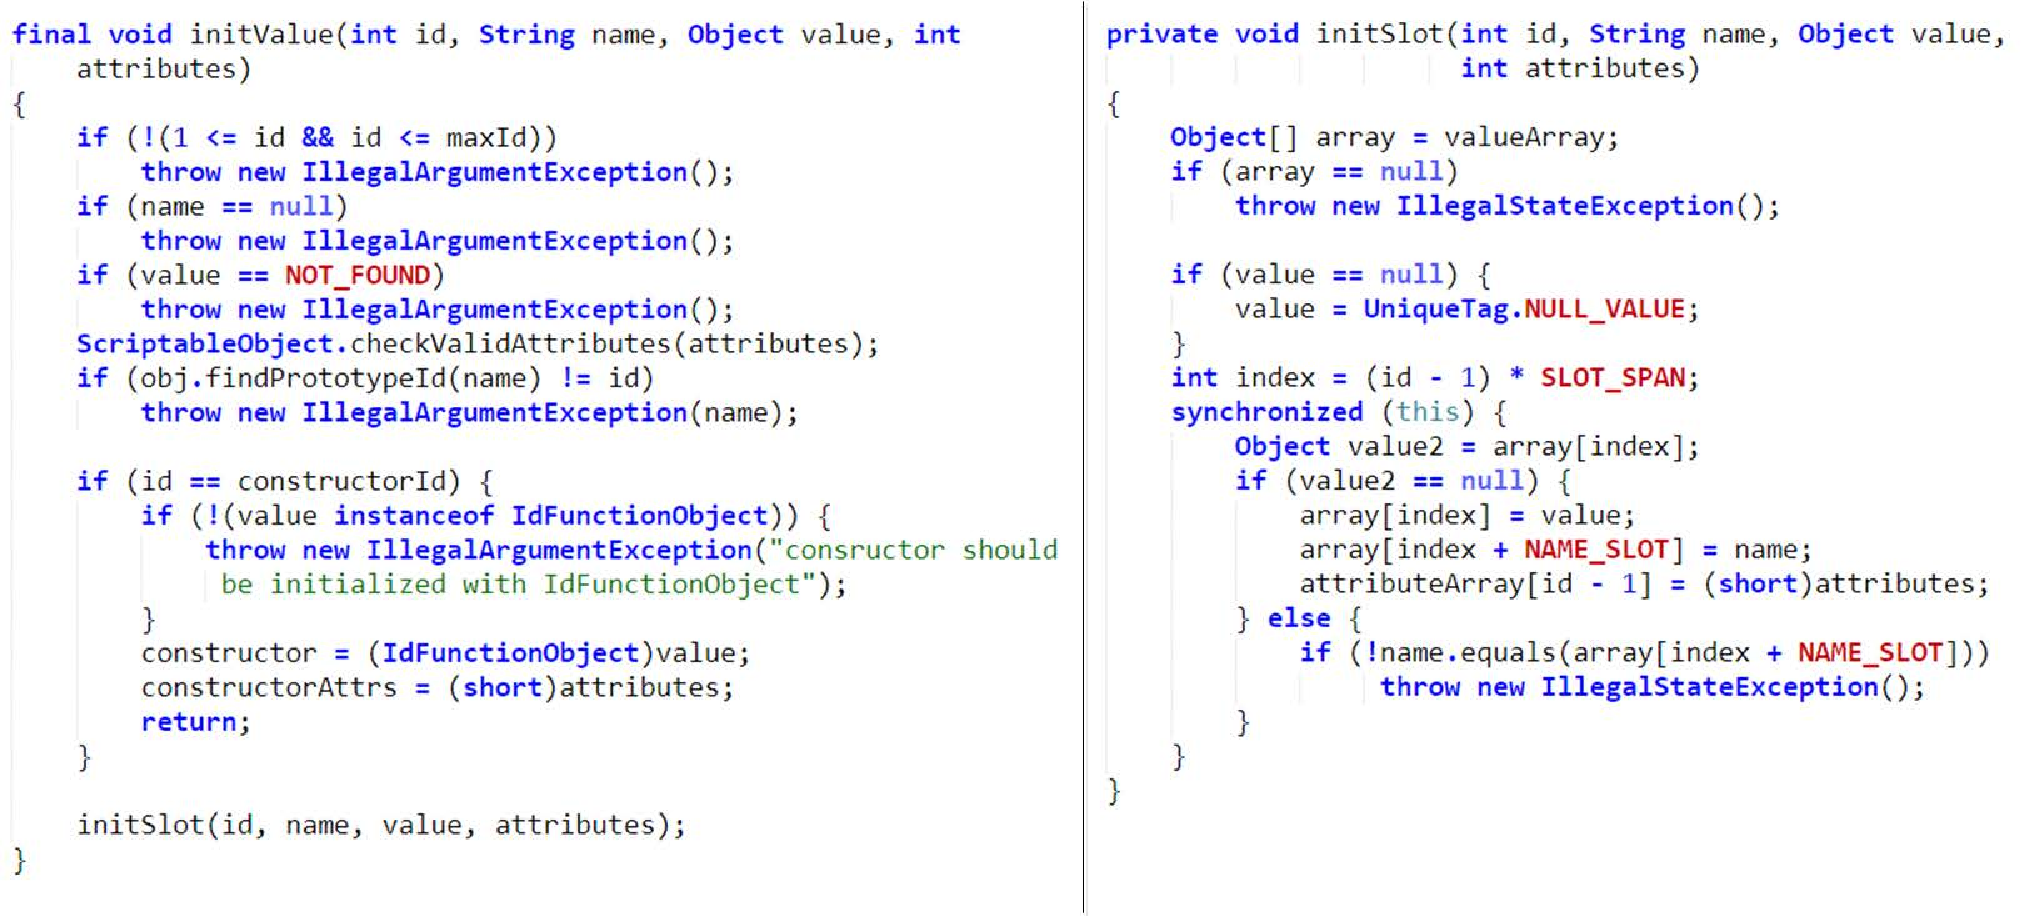
\includegraphics[width=16cm]{img/codeExample.pdf}
 \caption{\label{figure:sourceCodeExample}source code example}
\end{figure}

%\KZ{\textcolor{red}{Replace the above example with something a bit more complex but including
%all the features we have such as function call, comments, abbrev etc. It
%should contain several methods calling each other. Then you can show
%the call graph of them.}}


%\KZ{\textcolor[rgb]{1,0.1,0.1}{Label all the sections, figs and tables and refer to these labels in your
%text!}}

%\subsection{Parse Tree}

%\KZ{\textcolor{red}{The parse tree should be a simplified AST to save space. Right now, many of
%the nodes in the parse tree are redundant. E.g. you can use If (cond, thenpart,
% elsepart) to represent a if statement. Then recursively define the cond,
%thenpart and elsepart. The tree doesn't have to be the real Java parse but
%something that reflects the commonalities of all programming languages.}}

%\KZ{\textcolor{red}{Also simplify the description of the parse tree. Omit implementation details
%such as JavaParser. This work should not be limited to Java code only even
%we only evaluated on java repos.}}

%The first problem that we have to solve is how to represent source code. The basic format of source code is string, but we can't catch any structural information from it. However, parse tree holds much structural information because of its tree structure, so parse tree is a good choice to represent the structural information of code.
%When source code compiler compiling a source code file, it convert the source code into a sequence of tokens and then establish a parse tree to represent the code. So the parse tree can tell us much information about the structure of source code.
%\subsubsection{Original Parse Tree}
%We use the java library called JavaParser to establish the parse tree of Java code. And because we use JavaParser, the programming language mentioned in this paper is Java language. With the help of JavaParser we can create the parse tree as Fig \ref{figure:parseTree1} shows. And Fig \ref{figure:sourceCodeExample} is the source code example of Fig \ref{figure:parseTree1}.
%Fig \ref{figure:parseTree1} is the original parse tree of method ``initValue'' in Fig \ref{figure:sourceCodeExample}
%And our algorithm can be applied to all programming languages.
%and the suspension points in figure mean there are some other nodes here and we don't show it to save space, readers should complete these parts when implementing the parse tree.
%\begin{figure}[!htp]
% \centering
% 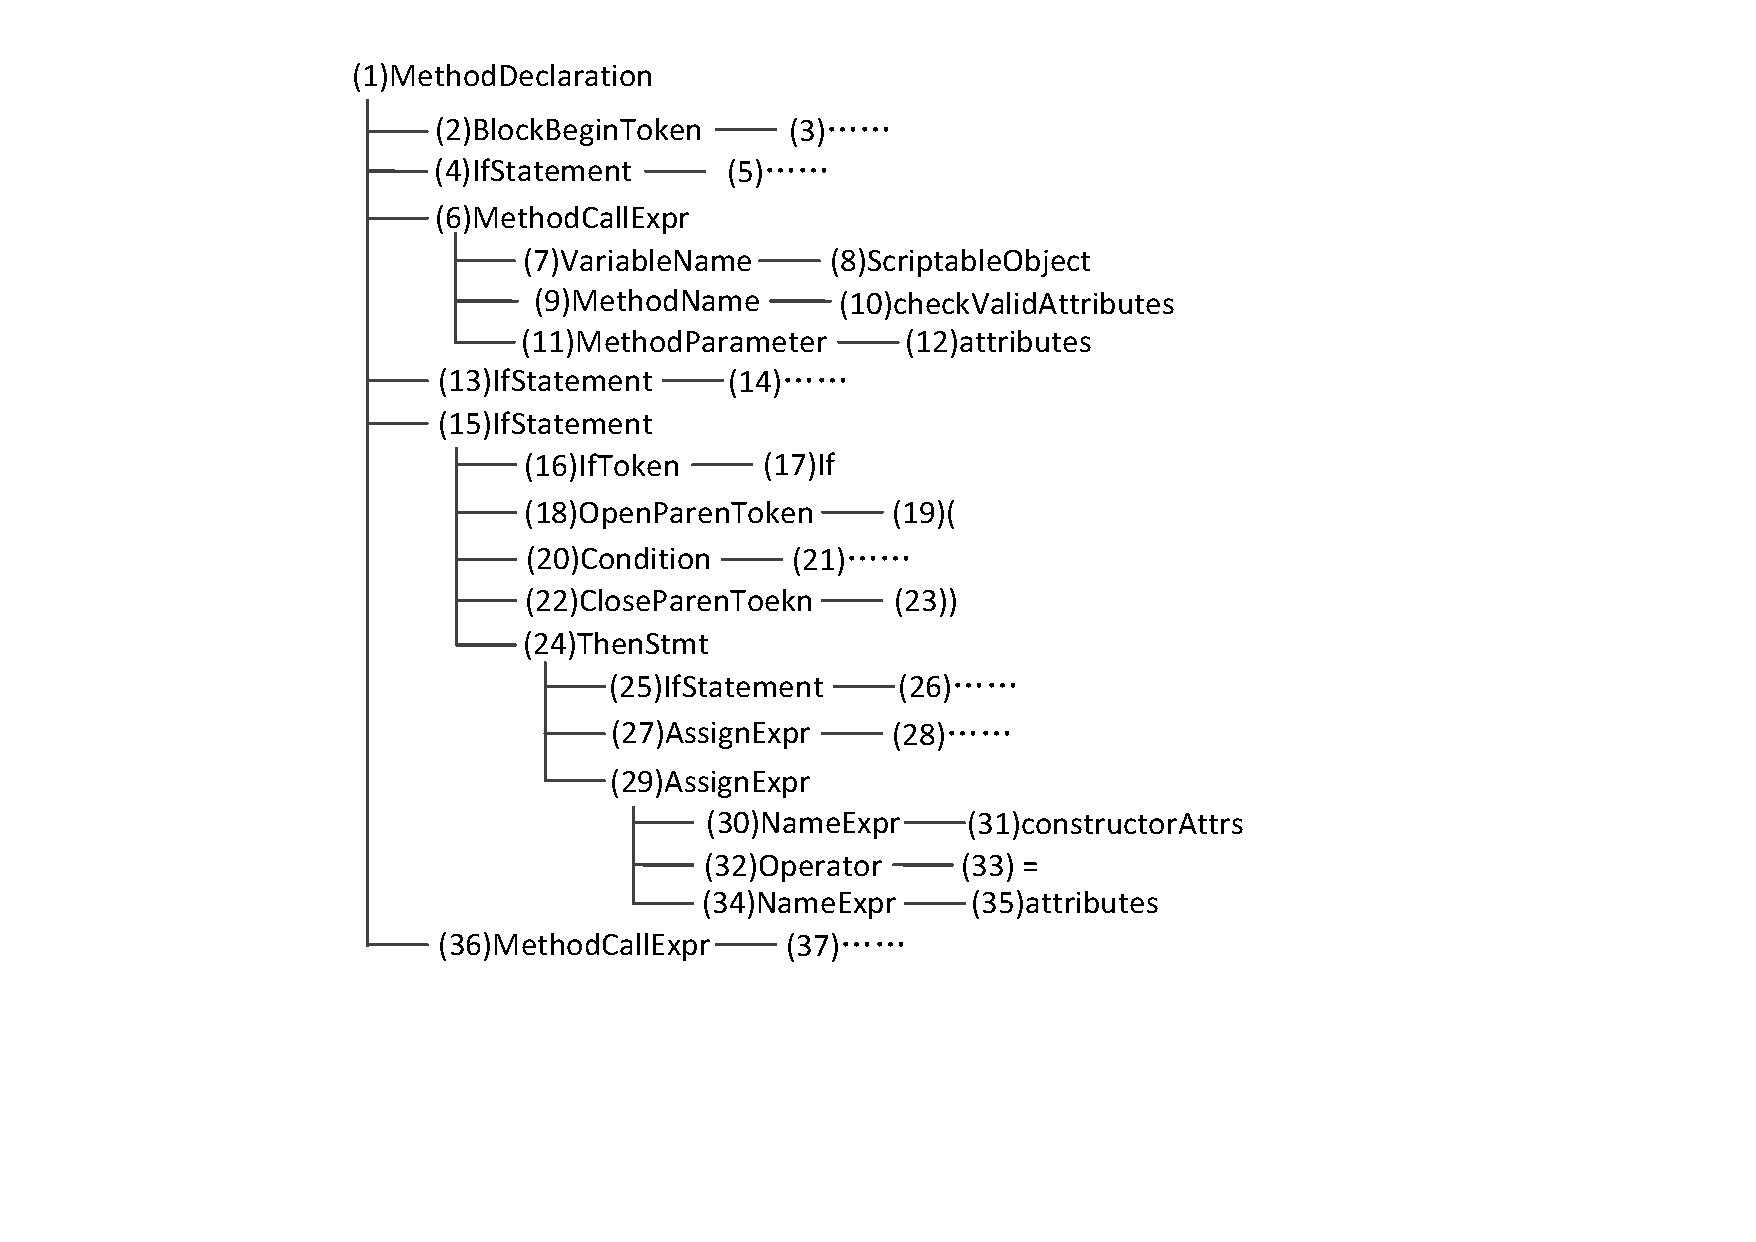
\includegraphics[width=0.8\linewidth]{img/parseTree1.pdf}
% \caption{\label{figure:parseTree1} original parse tree}
%\end{figure}

%\subsubsection{Our Parse Tree}\label{sec:ourParseTree}
%Comparing with Fig \ref{figure:sourceCodeExample} and Fig \ref{figure:parseTree1}, there are many new internal nodes appear in the parse tree. These internal nodes are specific to the expression or statement of the source code.
%So internal nodes held much structural information. And leaf nodes of parse tree all appear in the string of source code, they are all separated from the sequence of tokens.
Fig \ref{figure:parseTree2} shows the partial parse trees  for two
statements from the method ``initValue'' in
Fig \ref{figure:sourceCodeExample}. These parse trees are modified
from the ones used in Allamanis et al.~\shortcite{allamanis2015bimodal},
to adapt to the characters of source code repositories.

%If we want to know the topic of one method we must know the topic of other called methods.
%that are called by this function.
%Like two methods
In Fig \ref{figure:sourceCodeExample}, since ``initValue'' calls
``initSlot'', to correctly model the meaning of ``initValue'', one needs to
know the meaning of ``initSlot'' as well. This is the intuition behind using
the call graph information in our work. To this end, we replace the
called method name in parse tree by the topic represention of method.
That representation is a vector (e.g., $V_{checkValidAttribute}$),
similar to word embedding, calculated
from the parse tree of the called method (e.g., ``initSlot''
in the parse tree of ``initValue'').

%\KZ{\textcolor{red}{Change the following discussion once you change the example.}}
We also note that variable name ``constructorAttrs" in Fig~\ref{figure:parseTree2} isn't a real English word but combined by ``constructor" and ``attrs". If we use ``constructorAttrs" directly, we can't catch the topic of this variable exactly. So we split ``constructorAttrs" into ``constructor" and ``attrs", and add a new internal node called ``CombinedName". This new internal node means there is an identifier and it is combined by the children of this node. Meanwhile, ``attrs" isn't a real English word either. The word ``attrs" is an abbreviation of the word ``attributes", so we use ``attributes" instead of ``attrs". Now, in our new parse tree, we use ``constructor" and ``attributes" to replace ``constructorAttrs".
 %Readers can read more details in Section Identifier Semantics.%\ref{sec:identifier}
%about the process of identifiers.

% Finally, the bold and lean nodes in Fig \ref{figure:parseTree2} are changes of parse tree and $V_{checkValidAttributes}$ is the topic vector of method ``checkValidAttributes''.

\begin{figure}[ht]
 \centering
 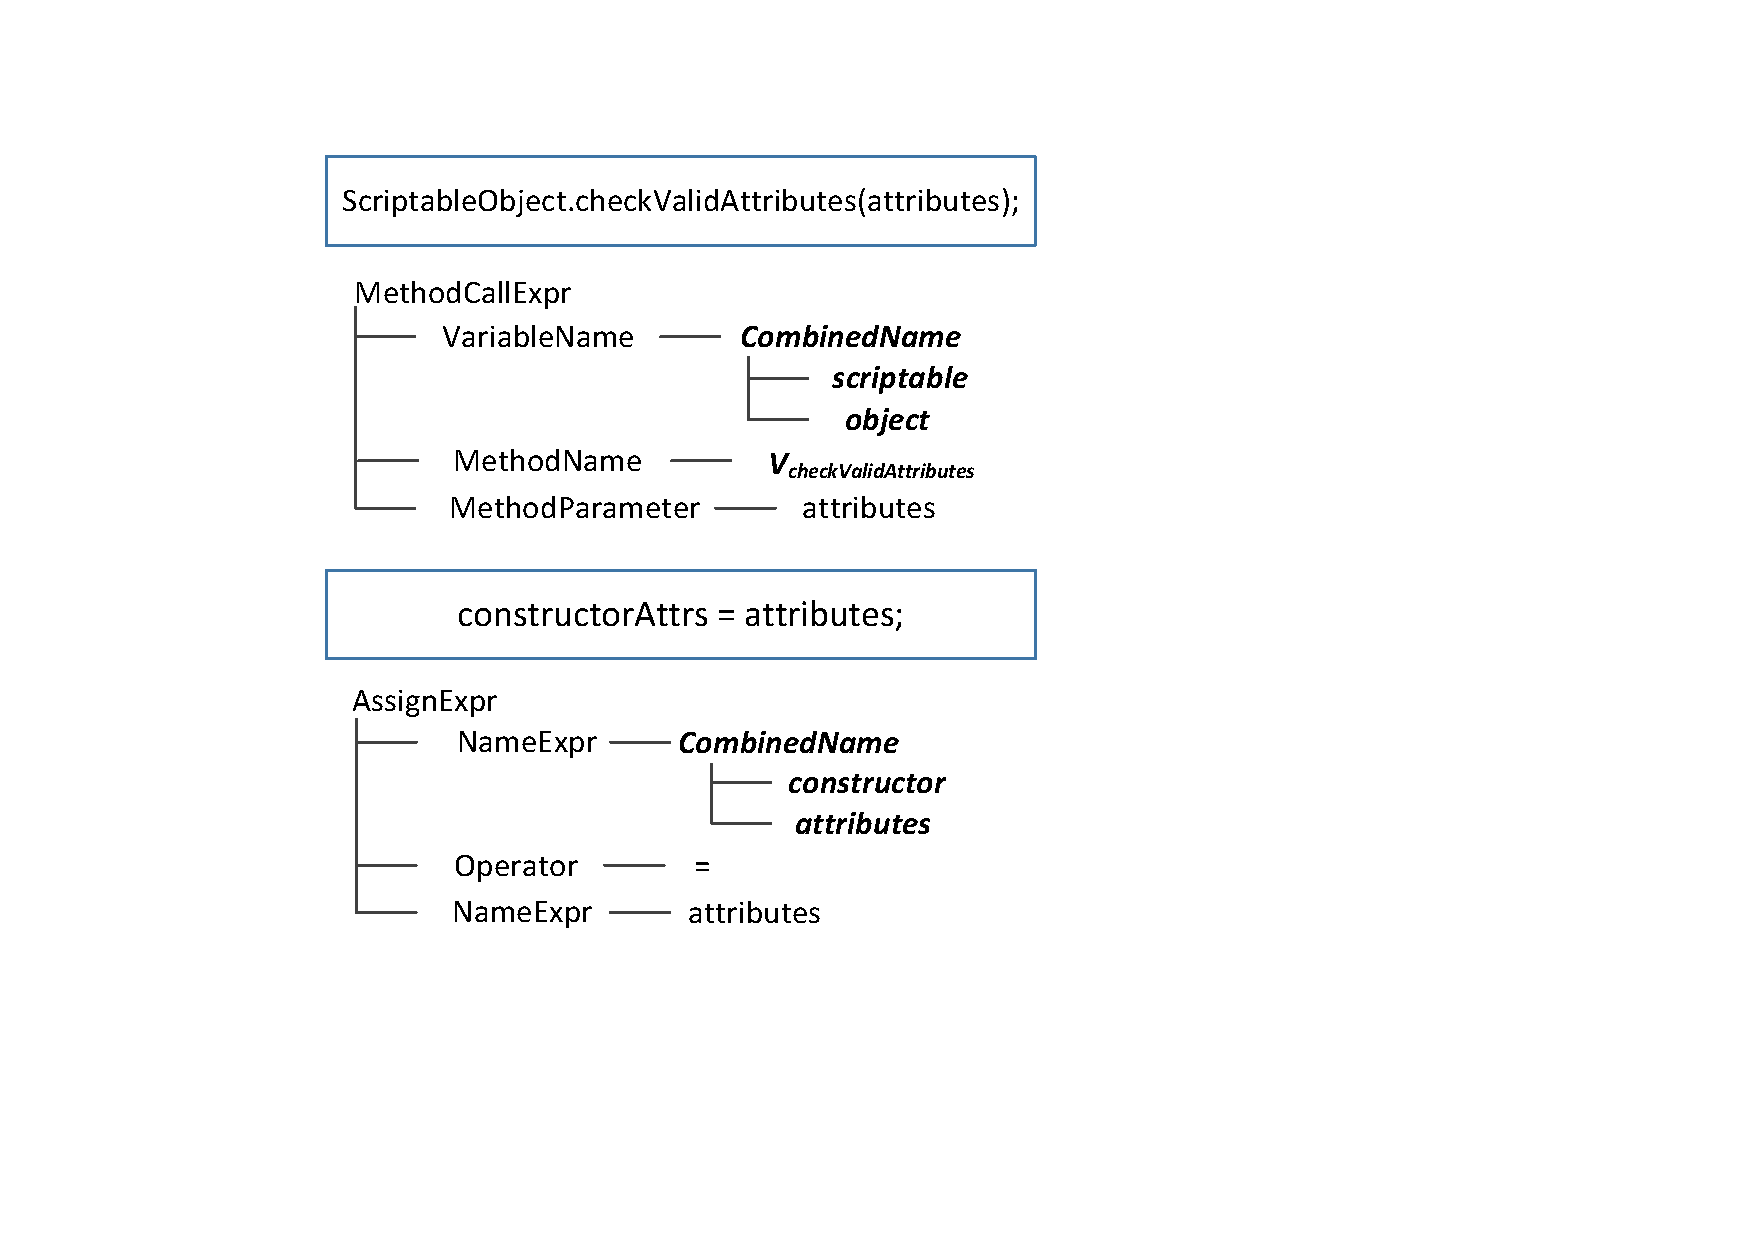
\includegraphics[width=0.6\linewidth]{img/newParseTree.pdf}
 \caption{\label{figure:parseTree2} parse tree}
\end{figure}

%\begin{figure}[!htp]
%\footnotesize{
% $~~~~~~~~~~~~~$   int getBufferSize(int bufferSize)\{\\
% $~~~~~~~~~~~~~$  $~~~~$   if (bufferSize $>$ 0)\\
% $~~~~~~~~~~~~~$  $~~~~~~~~$     return read();\\
% $~~~~~~~~~~~~~$  $~~~~$    else\\
% $~~~~~~~~~~~~~$  $~~~~~~~~$      return 0;\\
% $~~~~~~~~~~~~~~$   \}
% }
%    \caption{\label{figure:functionExapmle} function example}
%\end{figure}

\subsection{Call Graph}

%\KZ{\textcolor{red}{Tone down java... This paper is not only for java! Avoid the use of
%``as we all know..'' etc. Show the call graph of the running example.
%And that is it! Everybody understands it.}}

%\KZ{\textcolor{red}{The following para sounds like implementation details. Present only
%principle stuff here.}}

%Call Graph is one representation of invocation information in the source code repositories.
%The good running of repositories is based on the good running of every methods.
%And the whole repository is constructed over the calling of all methods in the repository. So call graph can help us mine more useful information of source code repository

In our approach, we replace the method name with its vector representation.
At training time, we will update this vector according to a global order of
function calls. After constructing the call graph, we can obtain the
topology sort of this graph and hence the calling order that we need.
Fig \ref{figure:callGraph} is the call graph of
Fig \ref{figure:sourceCodeExample}, and the calling order is
``checkValidAttributes'', ``IllegalArgumentException'', ``IllegalstateException'', ``initSlot''  and ``initValue''.
%To utilize invocation information, we have to generate call graph between all methods. As we all know, every java file is a java class and every java class has its own package name and many classes that it import.We firstly utilize the information of package name and import to generate the full name of every method. For example, if method A was called like a.A() and a is the objective of class com.github.abc.ClassA, then the method A's full name is com.github.abc.ClassA.A. And we can know the variable a's class's full name from package name and import information. In one word, the format of method's full name is (Package Name).(Class Name).(Method Name). In the previous example, com.github.abc is package name, ClassA is class name and A is the method name.

%After generating full name for every method, we can begin to build the call graph of all methods in the source code repository. For example, if method B is called in method C, there will be a direct edge from B to C. When we look through all methods in the repository we can build the call graph, and this call graph can be used to improve the performance of parse tree. And Fig \ref{figure:callGraph} is an example of call graph.
%\KZ{\textcolor{red}{Better use the running example here. You can
%simplify the names of the methods to save space.}}

\begin{figure}[ht]
 \centering
 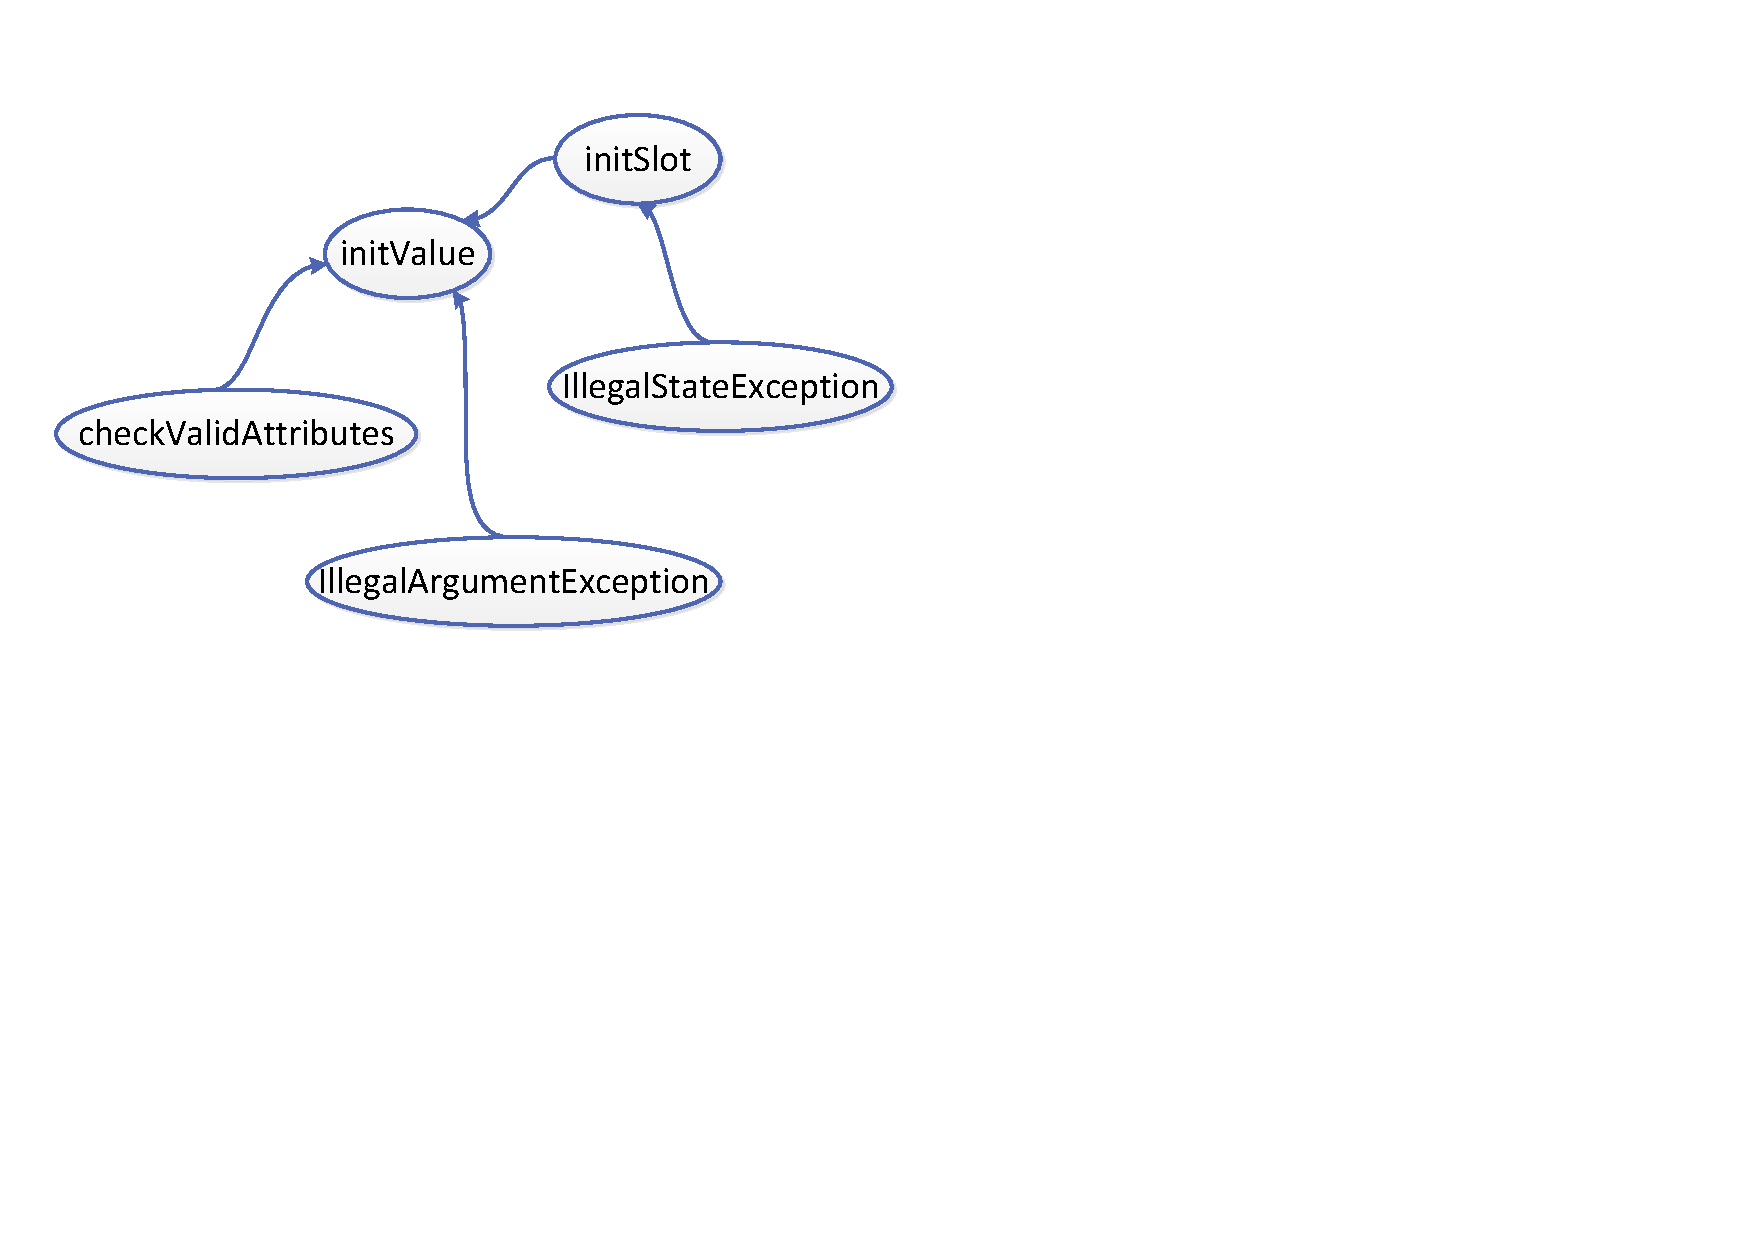
\includegraphics[width=0.7\columnwidth]{img/callGraph.pdf}
 \caption{\label{figure:callGraph} Call Graph Example}
\end{figure}

\subsection{Identifier Semantics}\label{sec:identifier}
%\KZ{\textcolor{red}{This section needs to be expanded significantly. I still don't understand
%Table \ref{table:abbr}. If you use rules, you should explicitly say what those
%rules are to recover the original words from the abbreviations. If you use
%some algorithm, better include the listing of the pseudo-code.}}

\begin{table}[ht]
\centering
\scriptsize{
\caption{\label{table:splitID} Example of Split Identifiers}
\begin{tabular}{|c|c|}
\hline
Identifier & Words \\
\hline
contextInitialize & context, initialize\\
\hline
apiSettings & api, settings\\
\hline
buildDataDictionary & build, data, dictionary\\
\hline
add\_result & add, result\\
\hline
\end{tabular}
}
\end{table}

\begin{table}[ht]
\centering
\scriptsize{
\caption{Example of Abbreviation}
\label{table:abbr}
\begin{tabular}{|c|c|c|}
\hline
Abbreviation & Origin & Context\\
\hline
val & value & key.value()\\
\hline
cm & confusion, matrix & new ConfusionMatrix()\\
\hline
conf & configuration & context.getConfiguration()\\
\hline
rnd & random & RandomUtils.getRandom()\\
\hline
\end{tabular}
}
\end{table}

In this work, we adopt two ways that extract the semantics from the identifiers.
One is to split all the long forms to multiple words and
the other one is to recover the full words from abbreviations.

Table \ref{table:splitID} shows some example identifiers and the results
of splitting. Many identifiers in the source code are combination of English words,
with the first letter of the word in upper case, or joined together using
underscores. We thus define simple rules to extract the original
English words accordingly.
%Firstly, we split all the combined phrases, which exist in the type or
%the assignment expression, to some independent words.
%All the words coming from one phrase are put in one list.
%The rule we apply to split words is simple. People usually use the alternation
%of upper cases and lower cases to combine two words and form a phrase.
%Sometimes the underscores are also used to segment two words.
%We just split the phrases according these rules. In the example,
%we split the type ``Matrix'' into a list which contains only one word
%``matrix'' and
For example, we can split the expression ``DoubleMatrix(confusionMatrix)''
into two lists. The first list contains ``double'' and ``matrix'',
and the second contains ``confusion'' and ``matrix''.

%For example, when we name a parameter whose function is to add two integers, we can name it as ``addScore'',
%changing the first letter of the second word to a capital one. When we encounter an identifier, we can search the alternation of capital and small letters, or
%observe the appearance of underscores.

Table \ref{table:abbr} shows some abbreviations and
their original version. We can infer the complete words by
looking for longer forms in the context of the identifier in the code.
Specifically, we compare the identifier with the word list generated from
the context of the identifier to see whether the identifier's name
is a substring of some word from the list, or is the combination of
the initial of the words in the list.
If the list contains only one word, we just check if the identifier
is part of that word. If so, we conclude that the identifier is the
abbreviation of that word with higher probability.
In the second situation, we can collect all the initials of the words
in the list together to see whether the identifier is part of
this collection. Suppose the code fragment is

\begin{lstlisting}
Matrix dm = new DoubleMatrix(confusionMatrix);
\end{lstlisting}
%After this process we can get most of the full names of the parameters.
We search for the original words of ``dm'' as follows.
At beginning, we see ``dm'' is not the substring of any word in any list
we establish. Then we collect the initials of the words in one list and
get three collections ``m'' ``dm'' and ``cm''.
Consequently, ``dm'' is an abbreviation of ``DoubleMatrix''.

%\textcolor{red}{
%Here let's talk about how we find out such original information from the abbreviations. As many programmers doing in their works,
%many parameters are named according to its type or assignment expression. So we get the original version of the parameter through its definition. We use the following definition statement.
%source code in Fig \ref{figure:indentifier} as an example.
%}

%\begin{figure}[!htp]
% \centering
% \caption{\label{figure:indentifier} Identifier Example}
%\end{figure}
%\textcolor{red}{Matrix dm = new DoubleMatrix(confusionMatrix);
%}

%\textcolor{red}{
%}

%\textcolor{red}{
%}

%According to the description in last section, some names of identifiers are phrases, which are meaningless since they are combined by
%two or more meaningful words together. They are quite important since they are the semantic information in this parse tree, showing the objective of why
%they are creative or what problems they solve. So we want to utilize such kind of information, instead of just keep the combination of them which makes no
%sense. There are two kinds of method to improve the semantic information. One is to split all the phrases to multiple words and the other one is to retrieve the
%full version from some abbreviated parameters.
%
%From Table \ref{table:splitID}, we see some examples of identifiers in source code. They are defined in the combination of some words, using the alternation of capital and small
%letters or splitting two words with a underscore. For example, when we name a parameter whose function is to add two integers, we can name it as ``addScore'',
%changing the first letter of the second word to a capital one. When we encounter an identifier, we can search the alternation of capital and small letters, or
%observe the appearance of underscores.
%
%Another situation is that many identifiers are also meaningless since they are the abbreviation of one or more words. Table \ref{table:abbr} shows some abbreviations and
%their original version. However, we can get their full name by checking their context. As we observed, we can split the context to words. Then, check the
%initials of these words to see whether they make up of the identifier we are operating. Take ``cm'' in Table \ref{table:abbr} as an example. When searching its context we can
%find ``confusion'' and ``matrix'', whose initials can make up of ``cm''. So we can believe the full version of ``cm'' is ``confusion matrix''.
%
%When parsing the code, adding such two kinds of operations can add more semantic information into the parse tree, which serves the goal that combining
%semantic and structural information together.

\subsection{Adding Comments}

%\KZ{may add preprocessing of comments if there's any theoretical value in there.}

Comments are often in natural language that provide valuable information
about the nearby code fragments. We therefore add comments into parse tree
as follows. Take the comment of method ``initSlot'' in
Fig \ref{figure:sourceCodeExample} as an example, and
Fig \ref{figure:nodeOfComment} is its representation in the parse tree.
We designate all words as children nodes of the new internal node ``Comment".
The node ``......'' indicates the other part of parse tree omitted from this
view.

%\begin{figure}[!htp]
%\footnotesize{
%\textcolor[rgb]{0,0,1}{// Maybe selected auto-focus but not available, so fall through here:}
%
%    \textcolor[rgb]{0.7,0.1,0.1}{if} (!
%    \textcolor[rgb]{0,0,1}{safeMode} \&\&
%    \textcolor[rgb]{0,0,1}{focusMode}
%     == \textcolor[rgb]{0.7,0.1,0.1}{null}) \{
%
%     $~~~~$
%        \textcolor[rgb]{0,0,1}{focusMode}
%         = findSettableValue(
%         \textcolor[rgb]{0,0,1}{"focus mode"},
%        \textcolor[rgb]{0,0,1}{supportedFocusModes},
%
%      $~~~~$
%        Camera.Parameters.\textcolor[rgb]{0,0,1}{FOCUS\_MODE\_MACRO},
%
%      $~~~~$
%        Camera.Parameters.\textcolor[rgb]{0,0,1}{FOCUS\_MODE\_EDOF});
%
%    \}
% }
%
% \caption{\label{figure:commentExample} comment example}
%\end{figure}

\begin{figure}[!htp]
 \centering
 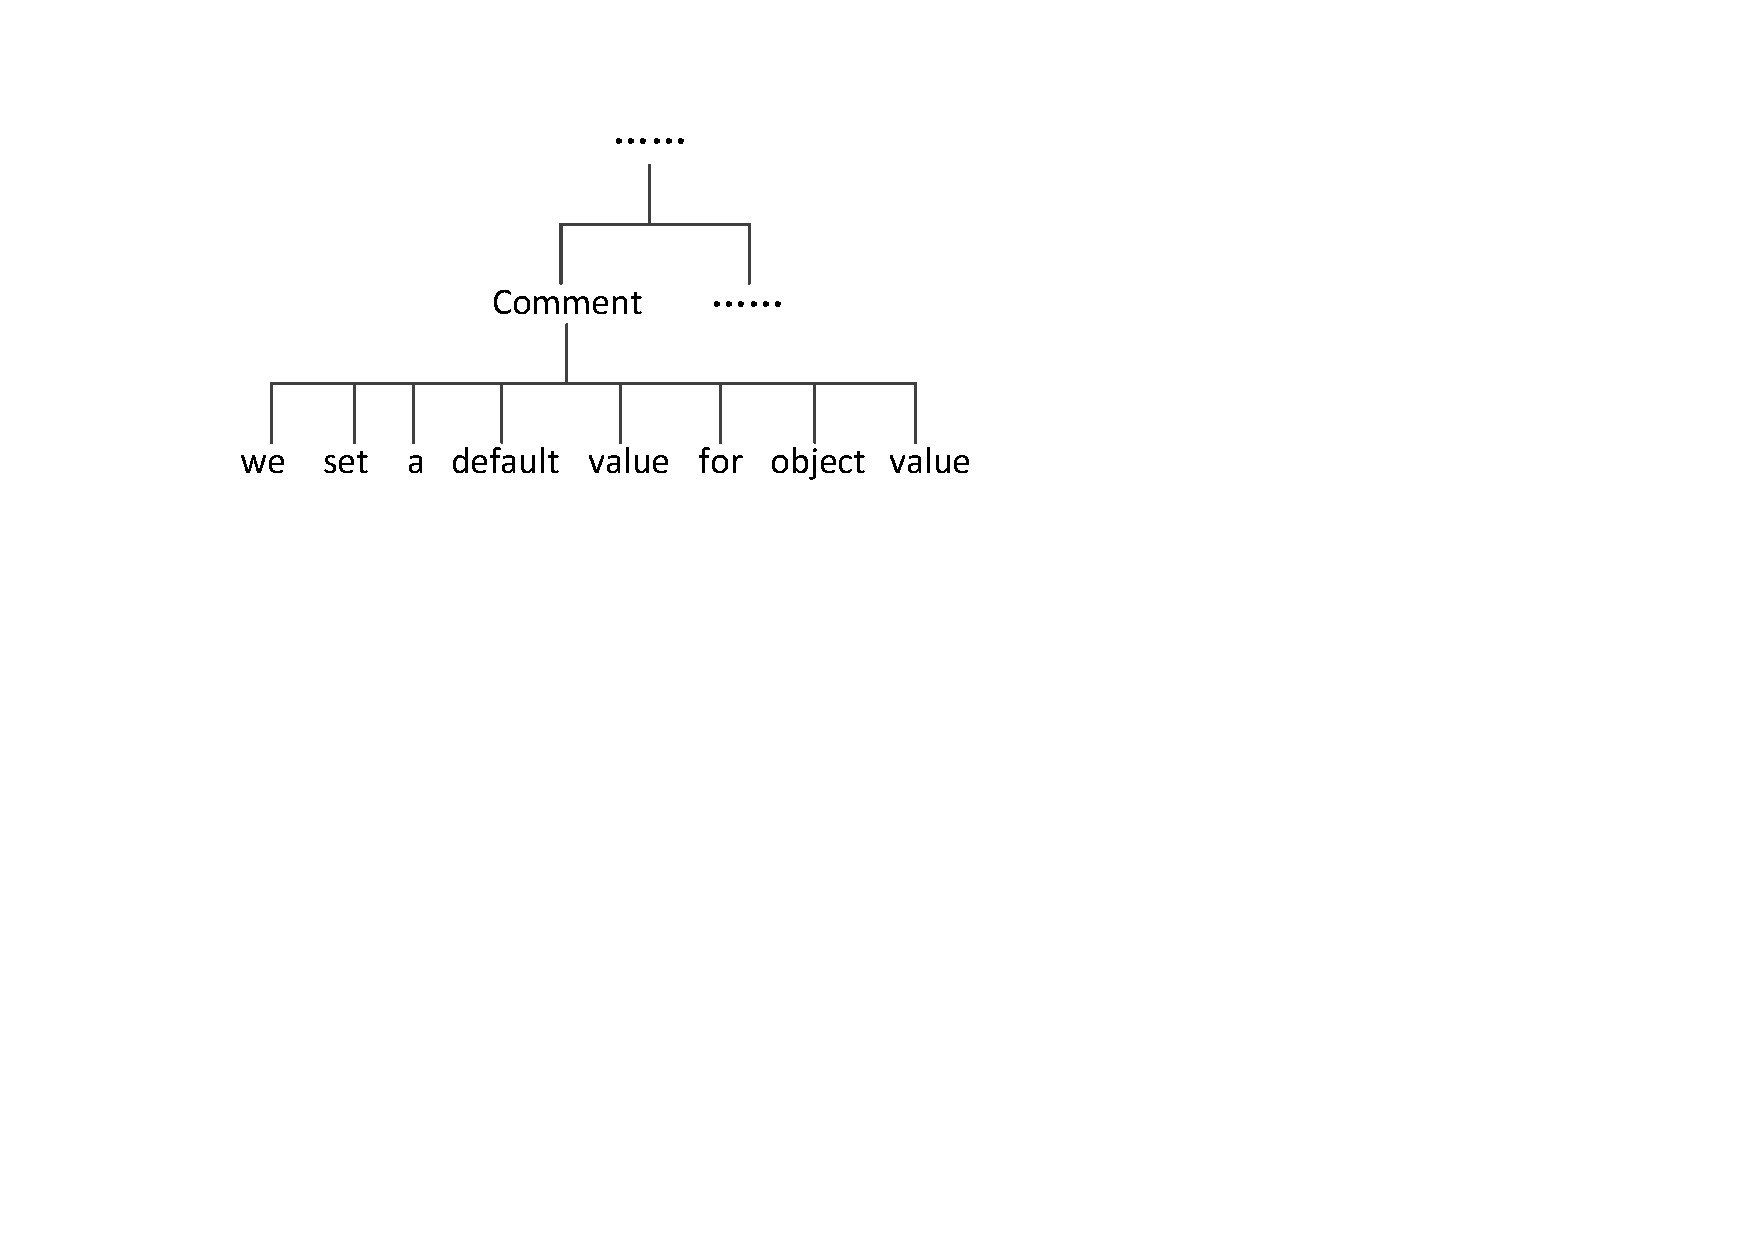
\includegraphics[width=0.7\linewidth]{img/comment.pdf}
 \caption{\label{figure:nodeOfComment} node of comments}
\end{figure}

%\subsection{Bimodal Modelling of Source Code and Natural Language}
%%\KZ{\textcolor{red}{This section relies too much on the ICML paper. You cannot assume
%%that the reader has read ICML 2015 before reading your paper.
%%Avoid citing ICML papers too many times (once will do!)
%%This section needs to be rewritten significantly.}}
%
%We joint source code functions and tags base on a bimodal model mentioned in~\cite{allamanis2015bimodal}.
%%Allamanis et al's model can be used to match source code snippets and natural language query. But the code snippets must has less than 300 words, while there are many functions that have more than 300 words in our model. And natural language query is also different from the tag. In our model, tags are many individual words and don't have any relationship with each other while training. But the words in the same query sentence must be trained together.
%
%%So we change some aspects of~\cite{allamanis2015bimodal} to make our model more suit to code repository and the new parse tree is one of changes.
%\subsubsection{Notation}
%We let $I$ be the set of internal nodetypes (not leaves) and $K$ be the set of tokens (leaf nodes). And a parse tree can be represented as $C\ =\ (Nd,ch,val)$ where $Nd=\{1,2,\cdots,N\}$ is set of all nodes($Nd=I\cup K$) and $ch$ is a function that map the node to its children nodes. $ch(1)=\{2,3\}$ means that node 2 and 3 is the children of node 1. The last one $val$ is a function that match the index of node and the value of this node. For example, $i$ is the index of node ``read", then val(i) equals to ``read". By the way, we index the nodes of parse tree by left-to-right depth first traversal of tree.
%%Fig \ref{figure:parseTree1} and Fig \ref{figure:parseTree2} shows some indexing examples.
%\subsubsection{Model Overview}
%We use a generative model to train our data. $P(C\ |\ T)$ is the probability of generating parse tree C on condition of the tag T. And our goal is to maximum this probability.
%\begin{equation}
%{
%    P(C\ |\ T)  = \prod_{n\in Nd:ch(n)\neq\phi}^N P(val(ch(n))\ |\ T,C_{\leq n}) \label{equa:probability}
%}
%\end{equation}
%Equation \ref{equa:probability} tells us how to calculate $P(C\ |\ T)$,
%%and it means if we want to generate a parse tree C based on tag T, we have to sequentially generate a child tuple for node n conditional upon the tag T and the partial tree $C_{\leq n}$.
%and $C_{\leq n}$ is the partial tree of $C$ that the index of all nodes are less than $n$.
%
%We also define $supp(i)$ and $S_{\theta}(v,T,C_{\leq n})$ to construct our model. $supp(i) = \{v\ :\ v=val(ch(n)) \bigwedge val(n)=i\ for\ some\ n\ in\ dataset\}$ is the set of all tuples that appear as the children of the node $i$. And we can convert scoring function $S_{\theta}(v,T,C_{\leq n})$ to probability by exponentiating and normalizing.
%\begin{equation}
%{
%    P(v|T,C_{\leq n})  = \frac{\exp s_{\theta}(v,T,C_{\leq n})}{\sum_{v^{'}\in supp(val(n))}\exp s_{\theta}(v^{'},T,C_{\leq n})}
%}
%\end{equation}
%where $\theta$ is the parameter of our model.
%
%\subsubsection{Scoring Function}
%The scoring function in our model is $s(v,T,C_{\leq n}) = (t \bigodot c)^{\top} r + b$ and $\bigodot$ is elementwise multiplication. $t$ is the representation vector of tag % that is unique to every word
% and c is the representation vector of partial parse tree $C_{\leq n}$. $r$ and $b$ are unique to each parent-children pair $(i,v)$ but $r$ is a vector and $b$ is a scalar number.
%
%Because the parse tree is always too complex to consider all nodes into scoring function, we just choose some nodes of parse tree as feature nodes to extract the representation of partial parse tree. And the two main features that we use are based on the 10 previous tokens following the indexing sort and 10 previous internal node types that in the path from node n to the root node. We let $c_{\varPhi_j}$ be the representation vector of one token that appears at $j$th position of all feature nodes and $H_j$ be the context matrix of $j$th feature node and the size of $H_j$ is $20\times20$. So that we can get c with the equation: $c=\sum_{j=1}^{J} H_{j} c_{\varPhi_j}$.
%
%All parameters appear in scoring function need to be trained and modified. And
%%we have to initialize all these parameters before begin training.
%we initialize them randomly around the center 0 with some small additive noise except $H_i$. We initialize $H_i$ as a diagonal matrix and the diagonals of $H_i$ are $\frac{1}{J} $, $J$ is the number of feature nodes and in our paper is 20.
%
%\subsubsection{Training}
%Our aim is to maximum $P(C\ |\ T)$, and because normalizing takes much time, we choose noise-contrastive estimation method \cite{gutmann2012noise} to train our model. The objective function can be written as in Mnih et al \cite{mnih2013learning}:
%\begin{equation}
%{
%\begin{split}
%  E_{(T,C_{\leq n},v)\sim D}[\log\Delta(\triangle s(v,T,C_{\leq n}))]\ + \\
%  kE_{(T,C_{\leq n},v^{'})\sim noise}[\log(1-\Delta(\triangle s(v^{'},T,C_{\leq n})))]
%\end{split}
%}
%\end{equation}
%where $d$ is the distribution of data, $nosie$ is the distribution of the noise data which is the posterior PCFG of the training data. And $k$ means that every pair $(T,C_{\leq n})$ has $k$ noise data.
%%And we choose the same initialization strategy as~\cite{allamanis2015bimodal} says.
%
%We also use AdaGrad method that is proposed by Duchi et al \cite{duchi2011adaptive} to gain better results.

%By the way, because we use invocation information, we need to sort all methods in one source code repository based on the call graph. And we decide to use the topology sort of the call graph, so that we can guarantee that when we meet a method in the parse tree we have get this method's newest representation vector. For example, there is a method initSlot was called by method initValue in Fig \ref{figure:sourceCodeExample}
%and the sequence of methods that are trained is initSlot and initValue. This sequence makes the representation vector of method initSlot is always the newest one when we calculate the vector of method initValue. And if there is a cycle in the call graph, we just break it randomly when generating topology sort.
